\documentclass{article}
\usepackage{graphicx}
\usepackage{easylist} 
\usepackage{url}
\usepackage{listings}
\usepackage{color}
\usepackage{pxfonts}
\usepackage{csquotes}
%\usepackage{mathtools}
\usepackage[colorlinks=true]{hyperref}

\hypersetup{
    colorlinks=true,
    linkcolor=blue,
    filecolor=magenta,      
    urlcolor=cyan,
    pdftitle={Sharelatex Example},
    bookmarks=true,
    pdfpagemode=FullScreen,
}



\definecolor{dkgreen}{rgb}{0,0.6,0}
\definecolor{gray}{rgb}{0.5,0.5,0.5}
\definecolor{mauve}{rgb}{0.58,0,0.82}
\definecolor{light-gray}{gray}{0.95}

\lstset{frame=tb,
  language=C++,
  aboveskip=6mm,
  belowskip=6mm,
  showstringspaces=false,
  columns=flexible,
  basicstyle={\small\ttfamily},
  numbers=left,
  numberstyle=\tiny\color{gray},
  keywordstyle=\color{blue},
  commentstyle=\color{dkgreen},
  stringstyle=\color{mauve},
  breaklines=true,
  breakatwhitespace=true,
  tabsize=3,
  basicstyle=\ttfamily,
  keywordstyle=\color{blue}\bfseries,
  showstringspaces=false,
  morekeywords={pTexture, pShader, pModel, pEntity, pScene, pProgram, pTexture2DRenderableDynamic, pTexture3D, pLightPoint, pLightSpot, pLightDirectional, pText, pCursor, pSkybox, GLfloat, GLint}
}

\begin{document}

\title{\textbf{Fillwave 4}
 - new OpenGL 3.3+ (OpenGL ES 3.0+) graphics engine for C++11 }
\author{Filip Wasil}

\maketitle

\begin{abstract}
Before you start please ensure your graphics card driver supports at least OpenGL 3.3 and GLSL 330 or OpenGL ES 3.0 and GLSL 300 ES. Also, your c++ compiler must support c++11 standard (Ex. g++\textgreater4.7 or clang++\textgreater3.3). PC Context examples provided are using GLFW3. Android context samples use are using EGL (Java and native). Of course you can use any stub you like (Ex. freeglut, qt or other).
\end{abstract}

\pagebreak
\tableofcontents

\newpage

\section{Introduction}
\subsection{Features}\label{sec:Features}
\indent \indent Graphics engine which you are about to use provides extremely, easy, portable, and uses C++11 modern API. It has all the essential functionalities that are needed to create a graphics layer for your application:

\begin{itemize}
  \item Physics buffers for each model.
  \item Skybox and terrain generation.
  \item Renderable textures support.
  \item Spot and directional light support (Point lights will be available soon).
  \item Ortographic and Perspective projections.
  \item Easy to use callbacks mechanism.
  \item Flexible and easy event system.
  \item Lots of examples and Doxygen documentation.
\end{itemize}

Probably you will ask how is Fillwave better than other, more extended engines out there. The answer generally depends on what is your target. With this engine you can easily build a graphics layer to any game without installing any large IDE or lots of libraries. Fillwave provides an abstraction layer to OpenGL API introducing minimum overhead. It does not rely on the OpenGL context you have, so it can be used with GLFW, Freeglut or even with QT as weel. The android example (Using \textbf{native app glue} and EGL directly) is also available.\newpage

\subsection{Code structure}\label{sec:Code structure}
\indent Files in this project are organized in simple manner:
\begin{itemize}
  \item "inc" - headers
  \item "src" - sources
  \item "doc" - documentation
  \item "ext" - sources of third party libraries (git submodules)
  \item "cmake" - cmake macros
  \item "examples" - multiplatform examples
  \item "scripts" - building scripts
\end{itemize}
\indent \indent Engine uses dual namespace design style for modules. Code is splitted into three namespaces: \textbf{fillwave}, \textbf{fillwave:framework}, \textbf{fillwave::core}. Core layer uses directly OpenGL driver API. \textbf{Framework} layer uses the \textbf{core} and by design implements a middleware of this project. The highest layer can be found under \textbf{fillwave} namespace. It is what we call Fillwave API. Naming convention is following:
\begin{itemize}
  \item "p" - shared pointer (Ex. pEntity)
  \item "pu" - unique pointer (Ex. puRenderer)
  \item "pw" - weak pointer (Ex. pwCameraPerspective)
  \item "e" - enumeration class (Ex. eDebuggerState)
  \item "I" - interface (Ex. IDrawable)
\end{itemize}

\subsection{Getting started}\label{sec:Getting started}
\indent \indent The basic application skeleton looks like:

\begin{lstlisting}
#include <fillwave/Fillwave.h>

using namespace fillwave;

int main(int argc, char* argv[]) {
   /* Create OpenGL/OpenGLES context */
   Engine* fillwave = new Engine(argc, argv);
   /* Create scene */
   /* enter rendering loop */
   delete engine;
   /* Delete OpenGL/OpenGLES context*/
   exit(EXIT_SUCCESS);
}
\end{lstlisting}

\subsection{Context creation}\label{sec:Context}
\indent \indent During the context initialization stage One must provide Fillwave engine a window (surface to draw on) and use \textbf{insert} functions in your context input handlers.

\begin{lstlisting}
void insertResizeScreen(GLuint width, GLuint height);
void insertInput(KeyboardEvent& e);
void insertInput(MouseButtonEvent& e);
void insertInput(ScrollEvent  & e);
void insertInput(CharacterEvent& e);
void insertInput(CharacterModsEvent& e);
void insertInput(CursorEnterEvent& e);
void insertInput(CursorPositionEvent& e);
void insertInput(TouchEvent& e);
void insertInput(TouchEvent& e);
\end{lstlisting}

\indent \indent Every time when there is an event incoming to you context, (Does not matter if you are using glfw, freegut, QT or other library) and you want Fillwave to handle it you should \textbf{insert} a proper event into the engine using \textbf{insertEvent} function. Above there is an example using GLFW. The \textbf{keyboardCallback} function was previously registered as keyboard callback in GLFW.  

\begin{lstlisting}

void ContextGLFW1::keyboardCallback(GLFWwindow* window,
                                   int key,
                                   int scancode,
                                   int action,
                                   int mods) {
   /* Create an event data and fill it */
   fillwave::framework::KeyboardEventData data;
   data.action = action;
   data.key = key;
   data.mode = mods;
   data.scanCode = scancode;
   
   /* Create an event */
   fillwave::framework::KeyboardEvent event(data);
   
   /* insert an event */
   mGraphicsEngine->insertInput(event);
}
\end{lstlisting}

\subsection{Rendering loop}\label{sec:Loop}

\indent \indent Last step that has to be done in order to use fillwave is rendering loop creation. In each iteration a \textbf{draw}, \textbf{drawLines}, or \textbf{drawPoints} function must be called with the \textbf{"How many seconds passed since last draw"} parameter. Also there is an extra \textbf{drawTexture} function which can display if a single texture in all You want to see. GLFW example of render loop will look like:

\begin{lstlisting}
void ContextGLFW1::render() {
   while (!glfwWindowShouldClose(mWindow)) {
      GLfloat timeSinceLastFrameInSec, now = glfwGetTime();

      timeSinceLastFrameInSec = now - mTimeExpired;
      mTimeExpired = now;
      mGraphicsEngine->draw(timeSinceLastFrameInSec);

      /* We were writing to back buffer - make it visible */
      glfwSwapBuffers(mWindow);
      
      /* evaluate GLFW input events */
      glfwPollEvents();
   }
}
\end{lstlisting}

\indent Offscreen drawing is possible using \textbf{capture} functions instead of \textbf{draw}.

\begin{lstlisting}
   void captureFramebufferToFile(const std::string& name);
   void captureFramebufferToBuffer(GLubyte* buffer,
                                   GLint* sizeInBytes,
                                   GLuint format,
                                   GLint bytesPerPixel);
\end{lstlisting}
\indent \indent If not sure about the format you want you can just leave the default parameters. \textbf{captureFramebufferToBuffer} will use \textbf{GL\_RGBA} with 4 bytes per pixel. This format is also a default one for \textbf{captureFramebufferToFile}.

\section{Digging into API}

\subsection{Entity}\label{sec:Entity}
\indent \indent \textbf{pEntity} is a base draw tree node. You can attach any other entities, models, particle emiters to it. You can move, rotate, and scale each of them.

\begin{lstlisting}
pEntity entity_parent = buildEntity();
pEntity entity_child = buildEntity();
entity_parent->attach(entity_child);
\end{lstlisting}

\indent \indent \textbf{pEntity} can be moved, rotated and scaled. The transformation matrix will be computed internally. However if one needs to set it directly (for example if it is computed by physics engine) there is a function provided:

\begin{lstlisting}
void setTransformation(glm::mat4 transformationMatrix);
\end{lstlisting}

\indent \indent Getting a transformation matrix is also possible:

\begin{lstlisting}
glm::mat4 getTransformation();
\end{lstlisting}

\subsection{Scene}\label{sec:Scene}
\indent \indent \textbf{pScenePerspective} (or \textbf{pSceneOrtographic}) by design is considered to be the root node of your \textbf{pEntity} tree. It stores its own \textbf{pCameraPerspective} (or \textbf{pCameraOrtographic}), \textbf{pSkybox} and \textbf{pCursor}. It also has an \textbf{onHide()} and \textbf{onShow()} virtual functions which will be execuded during scene change.

\begin{lstlisting}
/* Build scene */
pISceneOrtographic sceneO = buildSceneOrtographic();
pIScenePerspective speneP = buildScenePerspective();

/* Build camera */
pCameraOrtographic cO = std::make_shared<CameraOrtographic>();
pCameraPerspective cP = std::make_shared<CameraPerspective>();

/* Attach camera */
sceneO->setCamera(cO);
speneP->setCamera(cP);

/* Attach scene */
engine->setCurrentScene(sceneP);

\end{lstlisting}

\subsection{Camera}\label{sec:Camera}

\indent \indent There are two camera to chose from in Fillwave: \textbf{CameraPerspective} and \textbf{CameraOrtographic}.Providing empty quaternion results will make the camera look in \textbf{-Z} direction. Example camera creation is listed below:

\begin{lstlisting}
/* Perspective and ortographic cameras */
pCameraPerspective cameraP = std::make_shared<CameraPerspective>                
                    (glm::vec3(0.0,0.0,6.0), /* position */
                     glm::quat(), /* rotation */                
                     glm::vec3(0.0,1.0,0.0), /* head up direction */         
                     glm::radians(90.0), /* field of view angle */        
                     screenWidth/screenHeight, /* screen ratio */
                     0.1, /* projection near plane */
                     1000.0); /* projection far plane */
gCameraOrthographic cameraO = std::make_shared<CameraOrtographic> 
                        (glm::vec3(0.0,0.0,6.0),
                         glm::quat(), /* rotation */                
                         -10.0f, /* x left culling */
                         10.0f, /* x right culling */
                         10.0f, /* y up culling */
                         -10.0f, /* y down culling */
                         0.1f, /* z near culling  */
                         1000.0f); /* z far culling */
\end{lstlisting}

\subsection{Renderers}\label{sec:Renderers}

\indent \indent In current revision (4.0.0) there are two types of renderers - \textbf{Forward renderer} (RendererFR) and Program Based Render Pass renderer (RendererPBRP). Default one is \textbf{RendererFR}. Which one You will use is up to you. There is also third one coming out soon - \textbf{Deferred Renderer} RendererDR. Currenty it is only available for testing purposes. Each scene has its won renderer and can be set using \textbf{voi IScene::setRenderer(IRenderer)} function call;


\subsection{Programs and Shaders}\label{sec:Programs and Shaders}
\indent \indent Default programs can be built using \textbf{ProgramLoader} class using \textbf{getDefault} and \textbf{getDefaultBones} functions. See the example below:

\begin{lstlisting}
/* Create loader, and use it to create programs */
loader::ProgramLoader loader(gEngine);
pProgram default = loader.getDefault();
pProgram animation = loader.getDefaultBones();
\end{lstlisting}

\newpage

\subsection{Store functions}\label{sec:store functions}
\indent \indent Use \textbf{"store"} functions to create OpenGL objects which will be also stored by internal managers, and which will be internally, reloaded and reused if needed. Use store functions everywhere where possible.

\begin{lstlisting}
/* Store the shaders providing source file path */
pShader  storeShaderFragment(const std::string& path);
pShader  storeShaderVertex(const std::string& path);
pShader  storeShaderGeometry(const std::string& path);
pShader  storeShaderTesselationControl(const std::string& path);
pShader  storeShaderTesselationEvaluation(const std::string& p);

/* Store the shaders providing the source directly */
pShader  storeShaderFragment(const std::string& name, std::string& source);
pShader  storeShaderVertex(const std::string& name, std::string& source);
pShader  storeShaderGeometry(const std::string& name, std::string& source);
pShader  storeShaderTesselationControl(const std::string& name, std::string& source);
pShader  storeShaderTesselationEvaluation(const std::string& name, std::string& source);

pProgram storeProgram(const std::string& , std::vector<pShader>);

pTexture storeTexture (const std::string&, const GLuint&);
pTexture2DRenderableDynamic 
                       storeTextureDynamic (const std::string& fragmentShaderPath);
pTexture3D storeTexture3D(const std::string& path,
                          const std::string& path,
                          const std::string& path,
                          const std::string& path,
                          const std::string& path,
                          const std::string& path);

pLightSpot storeLightSpot(glm::vec3, glm::vec4, pEntity);
pLightPoint storeLightPoint(glm::vec3, glm::vec4, pEntity);
pLightDirectional storeLightDirectional(glm::vec4, glm::vec3);

pText storeText(std::string,std::string,GLfloat,GLfloat,GLfloat);

pCursor  storeCursor(pProgram, pTexture, GLfloat);
\end{lstlisting}

\newpage

\subsection{Model}\label{sec:Model}
\indent \indent Fillwave provides different methods to build a model. You can use \textbf{buildModel} functions or direct constructors.

\subsubsection{Direct methods}\label{sec:directCreation}

\begin{lstlisting}
/* 
 * When the appropriate map paths are available
 * together with your model asset file.
 */

pModel model = buildModel(engine, program, "model.obj");

pModel model = std::make_shared<framework::Model>(engine, program, "model.obj");

/*
 * When the appropriate map paths are available in your
 * file and you want to draw Your custom shape derived 
 * from framework::Shape<core::VertexBasic> 
 */

framework::Sphere sphere(1.0,10.0,10.0);

pModel model = buildModel(engine,
                          program,
                          sphere,
                          diffuseMap,
                          normalMap,
                          specularMap,
                          material);
                         
pModel model = std::make_shared<framework::Model>(engine,
                          program,
                          sphere,
                          diffuseMap,
                          normalMap,
                          specularMap,
                          material);
        
    
    
    
    
    
         
/* 
 * When we want to explicitily provide texture paths
 * but stll use the model asset from file.   
 */

pModel model = buildModel(engine,
                      program,
                      "model.obj",
                      "relativePathToDiffuseMap",
                      "relativePathToNormalsMap",
                      "relativePathToSpecularMap");
                      
pModel model = std::make_shared<framework::Model>(engine,
                       program,
                       "model.obj",
                       "relativePathToDiffuseMap",
                       "relativePathToNormalsMap",
                       "relativePathToSpecularMap");
                       
/*
 * When we want to use previously created texture
 * and material objects.
 */

pModel model = buildModel(engine,
                      program,
                      "model.obj",
                      diffuseMapTexture,
                      normalMapTexture,
                      specularMapTexture,
                      material);
pModel model = std::make_shared<Model>(engine,
                      program,
                      "model.obj",
                      diffuseMapTexture,
                      normalMapTexture,
                      specularMapTexture,
                      material);
\end{lstlisting}

\subsubsection{Builders}\label{sec:builderCreation}
\indent \indent Fillwave also provides two builders classes. You can use \textbf{BuilderModelExternalMaps} or \textbf{BuilderModelManual} described below.
\begin{lstlisting}
/* BuilderModelExternalMaps uses custom texture maps */

/* First method */
BuilderModelExternalMaps builder1 (engine,
                                   modelPath,
                                   pProgram program,
                                   diffusePath,
                                   normalPath,
                                   specularPath);

pModel m = builder1.build();

/* Second method */
BuilderModelExternalMaps builder1(engine);

pModel m = builder1.setModelPath(modelPath).
                  setProgram(program).
                  setdiffusePath(diffuseMap).
                  setNormalMapPath(normalsMap).
                  setSpecularMapPath(specularMap).
                  setMaterial(material).
                  build();



/* BuilderModelManual uses custom textures and material  *
/
/* First method */

BuilderModelManual builder2 (engine,
                             modelPath,
                             program,
                             diffuseMap,
                             normalsMap,
                             specularMap,
                             material);
pModel m = builder2.build();

/* Second method */

BuilderModelManual builder2 (engine);

pModel m = builder2.setModelPath(modelPath).
                  setProgram(program).
                  setDiffuseMapTexture(diffuseMap).
                  setNormalMapTexture(normalsMap).
                  setSpecularMapTexture(specularMap).
                  setMaterial(material).
                  build();

\end{lstlisting}

\indent In each case animations will be also loaded. You can check how many of them are available, and activate one You are interested in. Default value for active animation in each model is set to "FILLWAVE\_DO\_NOT\_ANIMATE".
\begin{lstlisting}
void setActiveAnimation(GLint animationID)
GLint getAnimations();
\end{lstlisting}

\subsubsection{Effects}\label{sec:Effects}
\indent \indent Fillwave provides \textbf{Effects} objects which can be added to each Model. You can use built in effects: \textbf{Fog}, \textbf{BoostColor}, \textbf{ClockwiseDrawEffect}, \textbf{Painter} and \textbf{TextureOnly}. You can also create Your own one by inheriting from \textbf{Effect} class and implementing all necessary methods. Remember that during the effect execution, the models program is already used, so You can call \textbf{uniformPush} function.

\begin{lstlisting}

pIEffect fog(new Fog());
pIEffect boost(new BoostColor(10.0));
pIEffect ccw(new ClockwiseDrawEffect());
pIEffect paint(new Painter());
pIEffect textureOnly(new TextureOnly());

model->addEffect(fog);
   
\end{lstlisting}

\subsection{Particles}\label{sec:Particles}
\indent \indent Particles system entry in Fillwave is in fact two (but powerfull) classes: \textbf{EmiterPointCPU} and \textbf{EmiterPointGPU}. The \textbf{EmiterPointGPU} particle emiter is computed entirely on GPU and uses Texture3D noise as a seed to generate random positions and velocities. It is slower but gives better robustness factors. \textbf{EmiterPointCPU} emiter particles are precomputed on CPU. They are faster but the factors are less robust.

\begin{lstlisting}
EmiterPointCPU::EmiterPointCPU(Engine* engine,
                                   GLfloat emitingSurfaceRadius,
                                   GLfloat robustness,
                                   GLint howMany,
                                   glm::vec4 color,
                                   glm::vec3 acceleration,
                                   glm::vec3 velocity,
                                   glm::vec3 distance,
                                   pTexture texture,
                                   GLfloat lifetimeInSec,
                                   GLfloat pointSize,
                                   GLboolean dephTest,
                                   GLfloat alphaCutOff)
                                   
pEmiterPointGPU::EmiterPointGPU(Engine* engine,
              GLfloat emitingSourceRate,
              GLuint howMany,
              glm::vec4 color,
              glm::vec3 acceleration,
              glm::vec3 startVelocity,
              glm::vec3 robustnessVelocity,
              glm::vec3 startPosition,
              glm::vec3 robustnessPosition,
              GLfloat startSize,
              GLfloat lifetime,
	          pTexture texture,
	          GLenum blendingSource,
	          GLenum blendingDestination,
	          GLboolean dephTest,
	          GLfloat alphaCutOff);

/* Change the blending function if needed */
/* Default blending source is GL_SRC_ALPHA */
/* Default blending destination is GL_ONE_MINUS_SRC_ALPHA*/
void setBlendingFunction (GLenum sourcePixel, GLenum destPixel);

\end{lstlisting}

\indent \textbf{EmiterPointCPU} emits particles using a round surface source. You can set the radius of this surface (\textbf{emitingSurfaceRadius}), and emiting \textbf{robustness}. \textbf{Robustness = 0} will make the particles flow perpendicular to the emiting surface. Parameter \textbf{dephTest} is critical. Using the depth test is slower but it guarantees that particles will stay visible only when they should be. Giving up the depth test will make them look much nicer and rendered faster, but they will be visible \textbf{always} which can make scene look not natural. AlphaCutOff parameter privides additional feature to discard all pixels with alpha value less than alphaCutOff.

\begin{figure}
    \centering
    \includegraphics[scale=0.17]{../../../fillwave-examples/screens/particles.png}
    \caption{Particles with depth test active}
    \label{particle_depth_test}
\end{figure}

\begin{figure}
    \centering
    \includegraphics[scale=0.17]{../../../fillwave-examples/screens/particles_b.png}
    \caption{Particles without depth test active}
    \label{particle_no_depth_test}
\end{figure}

\newpage

\subsection{Skybox}\label{sec:Skybox}

\indent \indent To create a skybox in fillwave You just need to provide texture paths as shown below.

\begin{lstlisting}

pTexture3D texture=pTexture3D(new Texture3D("textures_right.png",
                                              "textures_left.png",
                                              "textures_ceil.png",
                                              "textures_floor.png",
                                              "textures_front.png",
                                              "textures_back.png"));
pSkybox skybox = buildSkybox(engine,
                             texture);
scene->setSkybox(skybox);
\end{lstlisting}

\subsection{Terrain}\label{sec:Terrain}
\indent \indent Terrain in Fillwave can be generated using a voxel or quad chunks. These two methods provides complete mechanism for terrain generation.


\begin{lstlisting}
pShader fs = engine->storeShaderFragment("default.frag");
pShader vs = engine->storeShaderVertex("default.vert");
pProgram program = buildProgram(fs + vs);
pTerrain terrain = buildTerrainVoxel(engine,
                                  program,
                                  "textures/test.png",
                                  new terrain::MountainConstructor(),
                                  5);
gScene->attach(terrain);
\end{lstlisting}

\subsubsection{Voxel terrain}\label{sec:Voxel terrain}
\indent \indent To create a voxel terrain You should implement a derivative \textbf{VoxelConstructor} class, and implement a \textbf{calculateActive} method. The method will take coordinates of a Voxel in VoxelChunk and decide if it should be Active or not. Active Voxels will be drawn. More information can be found in \textbf{example\_terrain\_voxel} and \textbf{example\_terrain\_quad} examples.

\subsubsection{Mesh terrain}\label{sec:MeshTerrain}
\indent \indent To create a terrain Mesh you should create a class derived from \textbf{TerrainConstructor} class, and implement a \textbf{calculateHeight} method. The method should take x and z coordinates in the range of (-1,1) in and return Y position.

\subsection{Text}\label{sec:Text}
\indent \indent To create a 2D on screen text using ttf fonts You can use the \textbf{storeText} function.

\begin{lstlisting}
pText text = engine->storeText( "Hello Fillwave",/* content */
                                "FreeMono",/* font to use */
                                -0.95, /*left bottom y start (-1,1)*/    
                                -0.80, /*left bottom x start (-1,1)*/     
                                100.0, /* text size */
                                eTextEffect::none); /* text effect */
\end{lstlisting}

\indent \indent Fillwave will look for the font in the directory relative to Your binary directory. If it will not find it, it will search the \textbf{/usr/share/fonts/truetype/freefont/} directory. Next, it will create a texture and save its metadata. Finally this texture will be used as an atlas.

\subsection{Light}\label{sec:Light}
\indent \indent There are three Possible light types which can be created in Fillwave. These types are: point, spot and directional lights.

%\subsubsection{Ambient light}\label{sec:Ambient light}
%\indent \indent In current release ambient map are constant.

\subsubsection{Spot light}\label{sec:Spot light}
\indent \indent Spot lights have position, intensity (RGBA) and entity parameters. When the entity is provided, the light will follow the entity whatever happens and do not consider the \textbf{position}. When there is no entity provided, spot light will keep its position as set in constructor. Spot light generates perspective shadows into the scene.

\subsubsection{Directional light}\label{sec:Directional light}
\indent \indent Difference between spot and directional lights is a projection type. Directional lights will have an ortographic projection. It is perfect for light sources which gives constant size shadowing (Sun for example).

\subsubsection{Point light}\label{sec:Point light}
\indent \indent Point lights emits the light in all directions. In current revision this kind of light does not generate any shadowing effect.

\subsection{Logging}\label{sec:Logging}
\indent \indent All objects in Fillwave have a \textbf{log} function which prints most of the objects data to standard output. There are also predefined macros ready to use:

\begin{itemize}
\item \textbf{\textcolor{blue}{FLOG\_USER}} - free to use.
\item \textbf{\textcolor{gray}{FLOG\_CHECK}} - checks OpenGL errors.
\item \textbf{\textcolor{cyan}{FLOG\_INFO}} - prints \textbf{log} function information.
\item \textbf{\textcolor{yellow}{FLOG\_DEBUG}} - reserved for internal debug info.
\item \textbf{\textcolor{red}{FLOG\_ERROR}} - called in case of internal engine error.
\item \textbf{\textcolor{gray}{FLOG\_FATAL}} - just like FLOG\_ERROR but also calls abort(). It indicates blocking errors like: "Shaders not found". If such error occurs, and the reason is not trivial then it needs further investigation by the author. Do not hesitate to contact me in such case.
\end{itemize}
\indent To print a debug info in a certain source file You should define a module name and debug flags with macro \textbf{FLOGINIT}. Examples below:
\begin{lstlisting}

#define FLOGINIT_DEFAULT()
#define FLOGINIT_NONE()
#define FLOGINIT_MASK(FERROR | FFATAL | FDEBUG | FDEBUG | FUSER)
#define FLOGINIT("My module", FERROR | FFATAL | FDEBUG | FDEBUG | FUSER)


\end{lstlisting}


\newpage
\subsection{Event system}\label{sec:Event system}
\indent \indent There are two basic types of callback functions:
\begin{itemize}
\item hierarchy callbacks
\item private callbacks
\end{itemize}

\indent \indent \textbf Difference between the \textbf{hierarchy} and \textbf{private} is that hierarchy callback executes synchronously just before the draw when the scene is drawn. As opposite, the private one is called asynchronously when the particular event is introduced into the engine (Ex. Mouse button click, or Key press). Most commonly used \textbf{private callbacks} are \textbf{TimedCallback} classes:

\begin{lstlisting}
TimedCallback(GLfloat timeToFinish,
              EasingFunction easing = eEasing::None);
TimedScaleCallback(pEntity entity,
                   glm::vec3 normalizedScaleVec,
                   GLfloat lifetime,
                   EasingFunction easing);
TimedRotateCallback(pEntity entity,
                    glm::vec3 axis,
                    GLfloat angle,
                    GLfloat lifeTime,
                    EasingFunction easing);
TimedMoveCallback(pEntity entity,
                  glm::vec3 endPosition,
                  GLfloat lifeTime,
                  EasingFunction easing);
\end{lstlisting}

\indent \indent \textbf{TimedCallback} by itself stands only for a time delay. \textbf{TimedScaleCallback}, \textbf{TimedRotateCallback}, and \textbf{TimedMoveCallback} on the other hand can be used to modify the model scale/position/rotation in time with current easing described by std::function \textbf{EasingFunction}. Default easing for all of the callbacks is \textbf{LinearInterpolation}.
\newpage

\subsubsection{Focus functions and private callbacks}\label{sec:Focus functions and private callbacks}
\indent \indent Focus functionality and private callbacks were introduced to enable executing particular callbacks in particular entity without iterating over the whole scene tree. To set an entity which will receive a callback from chosen input \textbf{setFocus} functions should be used.
\newline

\begin{lstlisting}

void setFocus(eEventType eventType, pEntity entity);

\end{lstlisting}
   
\indent \indent To attach/detach an item callback to/from an entity:

\begin{lstlisting}
void Entity::attachHierarchyCallback(Callback* c);
void Entity::attachPrivateCallback(Callback* c);
void Entity::detachHierarchyCallback(Callback* c);
void Entity::detachPrivateCallback(Callback* c);
\end{lstlisting}

\subsubsection{Register, unregister and clear functions}\label{sec:register functions}
\indent \indent To register/unregister a callback in Fillwave use following functions:

\begin{lstlisting}
void registerCallback(Callback* c);
void unregisterCharacterModsCallback(Callback* c);
\end{lstlisting}

\indent \indent Note, that there is no need to \textbf{delete} any objects. This happens inside the callbacks.

\newpage

\subsection{Easing}\label{sec:Easing}

\indent \indent Timed Callbacks can be used to modify model transformation (scale, rotation and position) in time with particular easing. You can choose one of following easings define by \textbf{EasingFunction}:

\begin{center}

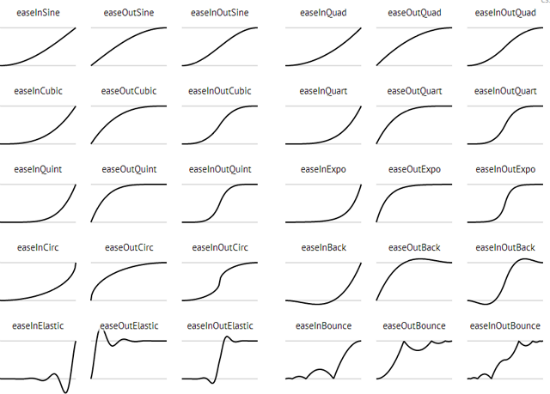
\includegraphics[scale=0.6]{easing.png}

\end{center}

\subsection{Physics}\label{sec:Physics}
\indent \indent To synchronize Your graphics with physics engine just use the \textbf{setTransformation} function which is available for each entity. it overwrites all other transformations for a model.

\begin{lstlisting}
void Entity::setTransformation(glm::mat4 modelMatrix)
\end{lstlisting}

\indent \indent If You have a light attached to Your model, the light will be moved together with its entity. However, only translation will be updated. If You want the light to keep the same rotation as its entity, You should use \textbf{updateParentRotation} function explicitily. 

\begin{lstlisting}
void Entity::updateParentRotation(glm::quat rotationQuaternion)
\end{lstlisting}

\indent \indent There is a \textbf{PhysicsMeshBuffer} defined. It can be used by physics engine to generate a collision object from a mesh polygons. Example usage of this buffer can be found in Fillwave car racing demo - \textbf{Waveracer}. To get physics buffer from asset file use:

\begin{lstlisting}
PhysicsMeshBuffer Engine::getPhysicalMeshBuffer(const std::string& shapePath)
\end{lstlisting}

\subsection{Extras}\label{sec:Extras}
\indent To change the background color use:

\begin{lstlisting}
void Engine::configureBackgroundColor (glm::vec3 color);
\end{lstlisting}

\indent To apply the time factor to in Fillwave engine use:

\begin{lstlisting}
void Engine::configureTime(GLfloat timeFactor); /* 1.0f as default */
\end{lstlisting}

\indent To get the current executable directory use:

\begin{lstlisting}
std::string Engine::getExecutablePath()
\end{lstlisting}

\indent To set/reset current "frames per seconds" counter in right left corner use:

\begin{lstlisting}
void Engine::configureFPSCounter(std::string fontName = "",
                            GLfloat xPosition = -0.95,
                            GLfloat yPosition = 0.95,
                            GLfloat size = 100.0);
\end{lstlisting}

empty or not valid font name will disable the FPS counter.

\indent To set/reset reset file logging use:

\begin{lstlisting}
void Engine::configureFileLogging(std::string fileName = "");
\end{lstlisting}

empty or not valid file name will disable the file logging.

\indent There are few texture generators built-in in Fillwave. To use them just pass one of the patterns as a texture path in \textbf{Model} constructor or \textbf{storeTexture} function:
\begin{lstlisting}
/* [R]_[G]_[B].color - for color texture */
/* [R]_[G]_[B].checkboard - for color checkboard texture */
/* "" - Black texture */

pModel model = buildModel(engine,
         programDefault,
         "model.obj",
         "255_0_0.checkboard", /* Red checkboard diffuse texture */
         "",  /* black normal map */
         "255_255_255.color"); /* white specular map */
\end{lstlisting}

\indent \indent Debugger related API is provided to enable simple debugging of depth maps from each spot light, and to enable viewing the pickable objects if there are any of them registered in the scene. debugger can be configured using one of the following enum constants. \textbf{toggleState} is a special value which will just iterate over the possible debugger configurations.

\begin{lstlisting}
enum class eDebuggerState {
   lightsSpot,
   lightsSpotColor,
   lightsSpotDepth,
   lightsPoint,
   lightsPointDepth,
   lightsPointColor,
   pickingMap,
   off,
   toggleState
};

void Engine::configureDebugger(eDebuggerState state);
\end{lstlisting}

\newpage

\section{Customization}

\subsection{Custom events}\label{sec:Custom events}
\begin{lstlisting}

namespace fillwave {
namespace actions {
struct NewEventData {
   int data;
   const eEventType type = eEventType::custom0; /* event ID */
};

class NewEvent: public Event<NewEventData> {
public:
   NewEvent();
   virtual ~NewEvent();
};
} /* actions */
} /* fillwave */
\end{lstlisting}
\subsection{Custom callbacks}\label{sec:Custom callbacks}
\begin{lstlisting}
namespace fillwave {
namespace actions {

class NewEngineCallback: public EngineCallback {
private:
   float mMaximimData;
   void sayHello() {FLOG_USER("Hello event");};
public:
   NewEngineCallback(eEventType eventType, float data);
   NewEngineCallback(float data);

   virtual ~NewActionCallback();
   void perform (Engine* engine, EventType* event);
   };

} /* actions */
} /* fillwave */
\end{lstlisting}
\subsection{Custom easing}\label{sec:Custom easing}
\textbf{TimedMoveCallbackCustom.h}
\begin{lstlisting}
namespace fillwave {
namespace actions {

class TimedMoveCallbackCustom: public fillwave::framework::TimedMoveCallback {
public:
   TimedMoveCallbackCustom(pEntity entity,
                           glm::vec3 endPosition,
                           GLfloat lifeTime);
   virtual ~TimedMoveCallbackCustom();
   GLfloat easeCustom(GLfloat progress);
};
} /* actions */
} /* fillwave */
\end{lstlisting}
\textbf{TimedMoveCallbackCustom.cpp}
\begin{lstlisting}
namespace fillwave {
namespace actions {

TimedMoveCallbackCustom::TimedMoveCallbackCustom(pEntity entity,
                                                 glm::vec3 endPosition,
                                                 GLfloat lifeTime):TimedMoveCallback(entity, endPosition,lifeTime, eEasing::Custom) {

}

TimedMoveCallbackCustom::~TimedMoveCallbackCustom() {

}

GLfloat TimedMoveCallbackCustom::easeCustom(GLfloat progress) {
   /* You custom easing function goes here. For example: */
   return QuinticEaseIn(progress)*QuinticEaseIn(progress);
}

} /* actions */
} /* fillwave */
\end{lstlisting}
%\subsection{Custom buffers}\label{sec:Custom buffers}
%\lstinputlisting[firstline=33,lastline=70]%{../../../fillwave/inc/fillwave/core/VertexBufferTerrain.h}

\section{Examples}

Basic example You can find below:
\lstinputlisting[firstline=33,lastline=200]{../../../fillwave-examples/src/example_simple/example_simple.cpp}

Basic example You can find below:
\newpage

\large

\href{https://github.com/filipwasil/Fillwave-examples}{Main example repository}
\newline\newline
\href{https://github.com/filipwasil/fillwave-examples/blob/master/src/example_text/example_text.cpp}{Example: Text} \newline
\href{https://github.com/filipwasil/Fillwave-examples/blob/master/src/example_animation/example_animation.cpp}{Example: Animation}
\newline
\href{https://github.com/filipwasil/Fillwave-examples/blob/master/src/example_callbacks/example_callbacks.cpp}{Example: Timed callbacks with custom easing}
\newline
\href{https://github.com/filipwasil/Fillwave-examples/blob/master/src/example_cursor_picking/PickableModel.cpp}{Example: Picking}
\newline
\href{https://github.com/filipwasil/Fillwave-examples/tree/master/src/example_dynamic_texture}{Example: Dynamic texture}
\newline
\href{https://github.com/filipwasil/Fillwave-examples/blob/master/src/example_effects/example_effects.cpp}{Example: Effects}
\newline
\href{https://github.com/filipwasil/Fillwave-examples/blob/master/src/example_normals_and_specular_map/example_normals_and_specular_map.cpp}{Example: Specular and normal maps}
\newline
\href{https://github.com/filipwasil/Fillwave-examples/blob/master/src/example_skybox/example_skybox.cpp}{Example: Skybox}
\newline
\href{https://github.com/filipwasil/Fillwave-examples/blob/master/src/example_shadow/example_shadow.cpp}{Example: Lights}
\newline
\href{https://github.com/filipwasil/Fillwave-examples/blob/master/src/example_particles/example_particles.cpp}{Example: Particles}
\newline
\href{https://github.com/filipwasil/Fillwave-examples/blob/master/src/example_terrain_quad/example_terrain_quad.cpp}{Example: Quad Terrain}
\newline
\href{https://github.com/filipwasil/Fillwave-examples/blob/master/src/example_terrain_voxel/example_terrain_voxel.cpp}{Example: Voxel terrain}
\newline
\href{https://github.com/filipwasil/Fillwave-examples/blob/master/src/example_impostor/example_impostor.cpp}{Example: Custom shader shape}
\newline
\href{https://github.com/filipwasil/Fillwave-examples/blob/master/src/example_post_processing/example_post_processing.cpp}{Example: Postprocessing}
\newline
\href{https://github.com/filipwasil/Fillwave-examples/blob/master/src/example_ortographic_projection/example_ortographic_projection.cpp}{Example: Ortographic projection}
\newline
\href{https://github.com/filipwasil/Fillwave-examples/blob/master/src/example_effects/example_effects.cpp}{Example: Effects}
\newline\newline
------------------------------------------------------
\newline
\href{https://github.com/filipwasil/fillwave-waveracer}{Waveracer game draft}
\newline
------------------------------------------------------
\newline\newline
\href{https://github.com/filipwasil/fillwave-android-activity}{Example: Android activity}
\newline
\href{https://github.com/filipwasil/fillwave-android-jni-lib}{Example: Android JNI library}
\newline
\href{https://github.com/filipwasil/fillwave-android-activity-native}{Example: Android pure native project}
\newpage
%\begin{equation}
%\label{eq:1}
%\sum_{i=0}^{\infty} a_i x^i
%\end{equation}

\section{Licenses}\label{sec:Licenses}
\begin{lstlisting}
/*************************************************************************
 * Fillwave C++11 graphics Engine
 * Copyright (C) 2015 Filip Wasil
 *  All Rights Reserved.
 * This library is available free of charge for any commercial
 * or non-commercial use. However, You are obligated to put
 * a clearly visible information in Your license agreement
 * that Your Software uses Fillwave library. Fillwave uses
 * few external libraries and their licenses are written below.
 * If You are interested in extra support, extra features
 * or cooperation I look forward to hearing from You.
 *
 *     Filip Wasil              fillwave@gmail.com
 */
 
 /* OpenGL
http://www.opengl.org/

* AssImp library
Open Asset Import Library (assimp)

Copyright (c) 2006-2012, assimp team
All rights reserved.

Redistribution and use of this software in source and binary forms, 
with or without modification, are permitted provided that the 
following conditions are met:

* Redistributions of source code must retain the above
  copyright notice, this list of conditions and the
  following disclaimer.

* Redistributions in binary form must reproduce the above
  copyright notice, this list of conditions and the
  following disclaimer in the documentation and/or other
  materials provided with the distribution.

* Neither the name of the assimp team, nor the names of its
  contributors may be used to endorse or promote products
  derived from this software without specific prior
  written permission of the assimp team.

THIS SOFTWARE IS PROVIDED BY THE COPYRIGHT HOLDERS AND CONTRIBUTORS 
"AS IS" AND ANY EXPRESS OR IMPLIED WARRANTIES, INCLUDING, BUT NOT 
LIMITED TO, THE IMPLIED WARRANTIES OF MERCHANTABILITY AND FITNESS FOR
A PARTICULAR PURPOSE ARE DISCLAIMED. IN NO EVENT SHALL THE COPYRIGHT 
OWNER OR CONTRIBUTORS BE LIABLE FOR ANY DIRECT, INDIRECT, INCIDENTAL,
SPECIAL, EXEMPLARY, OR CONSEQUENTIAL DAMAGES (INCLUDING, BUT NOT 
LIMITED TO, PROCUREMENT OF SUBSTITUTE GOODS OR SERVICES; LOSS OF USE,
DATA, OR PROFITS; OR BUSINESS INTERRUPTION) HOWEVER CAUSED AND ON ANY 
THEORY OF LIABILITY, WHETHER IN CONTRACT, STRICT LIABILITY, OR TORT 
(INCLUDING NEGLIGENCE OR OTHERWISE) ARISING IN ANY WAY OUT OF THE USE 
OF THIS SOFTWARE, EVEN IF ADVISED OF THE POSSIBILITY OF SUCH DAMAGE.



******************************************************************************

AN EXCEPTION applies to all files in the ./test/models-nonbsd folder.
These are 3d models for testing purposes, from various free sources
on the internet. They are - unless otherwise stated - copyright of
their respective creators, which may impose additional requirements
on the use of their work. For any of these models, see 
<model-name>.source.txt for more legal information. Contact us if you
are a copyright holder and believe that we credited you inproperly or 
if you don't want your files to appear in the repository.


******************************************************************************

Poly2Tri Copyright (c) 2009-2010, Poly2Tri Contributors
http://code.google.com/p/poly2tri/

All rights reserved.
Redistribution and use in source and binary forms, with or without modification,
are permitted provided that the following conditions are met:

* Redistributions of source code must retain the above copyright notice,
  this list of conditions and the following disclaimer.
* Redistributions in binary form must reproduce the above copyright notice,
  this list of conditions and the following disclaimer in the documentation
  and/or other materials provided with the distribution.
* Neither the name of Poly2Tri nor the names of its contributors may be
  used to endorse or promote products derived from this software without specific
  prior written permission.

THIS SOFTWARE IS PROVIDED BY THE COPYRIGHT HOLDERS AND CONTRIBUTORS
"AS IS" AND ANY EXPRESS OR IMPLIED WARRANTIES, INCLUDING, BUT NOT
LIMITED TO, THE IMPLIED WARRANTIES OF MERCHANTABILITY AND FITNESS FOR
A PARTICULAR PURPOSE ARE DISCLAIMED. IN NO EVENT SHALL THE COPYRIGHT OWNER OR
CONTRIBUTORS BE LIABLE FOR ANY DIRECT, INDIRECT, INCIDENTAL, SPECIAL,
EXEMPLARY, OR CONSEQUENTIAL DAMAGES (INCLUDING, BUT NOT LIMITED TO,
PROCUREMENT OF SUBSTITUTE GOODS OR SERVICES; LOSS OF USE, DATA, OR
PROFITS; OR BUSINESS INTERRUPTION) HOWEVER CAUSED AND ON ANY THEORY OF
LIABILITY, WHETHER IN CONTRACT, STRICT LIABILITY, OR TORT (INCLUDING
NEGLIGENCE OR OTHERWISE) ARISING IN ANY WAY OUT OF THE USE OF THIS
SOFTWARE, EVEN IF ADVISED OF THE POSSIBILITY OF SUCH DAMAGE.
* FreeType 2 library (FTL licence)
http://www.freetype.org/

  This  license  grants  a  worldwide, royalty-free,  perpetual  and
  irrevocable right  and license to use,  execute, perform, compile,
  display,  copy,   create  derivative  works   of,  distribute  and
  sublicense the  FreeType Project (in  both source and  object code
  forms)  and  derivative works  thereof  for  any  purpose; and  to
  authorize others  to exercise  some or all  of the  rights granted
  herein, subject to the following conditions:

    o Redistribution of  source code  must retain this  license file
      (`FTL.TXT') unaltered; any  additions, deletions or changes to
      the original  files must be clearly  indicated in accompanying
      documentation.   The  copyright   notices  of  the  unaltered,
      original  files must  be  preserved in  all  copies of  source
      files.

    o Redistribution in binary form must provide a  disclaimer  that
      states  that  the software is based in part of the work of the
      FreeType Team,  in  the  distribution  documentation.  We also
      encourage you to put an URL to the FreeType web page  in  your
      documentation, though this isn't mandatory.

  These conditions  apply to any  software derived from or  based on
  the FreeType Project,  not just the unmodified files.   If you use
  our work, you  must acknowledge us.  However, no  fee need be paid
  to us.

* GLEW library
http://glew.sourceforge.net/

GLEW is originally derived from the EXTGL project by Lev Povalahev. The source
code is licensed under the Modified BSD License, the Mesa 3-D License
(MIT License), and the Khronos License (MIT License). The automatic code
generation scripts are released under the GNU GPL. 

* Lanyon
Released under MIT License
Copyright (c) 2014 Mark Otto.

Permission is hereby granted, free of charge, to any person obtaining
a copy of this software and associated documentation files (the "Software"),
to deal in the Software without restriction, including without limitation
the rights to use, copy, modify, merge, publish, distribute, sublicense,
and/or sell copies of the Software, and to permit persons to whom
the Software is furnished to do so, subject to the following conditions:

The above copyright notice and this permission notice
shall be included in all copies or substantial portions of the Software.

THE SOFTWARE IS PROVIDED "AS IS", WITHOUT WARRANTY OF ANY KIND,
EXPRESS OR IMPLIED, INCLUDING BUT NOT LIMITED TO THE WARRANTIES OF MERCHANTABILITY,
FITNESS FOR A PARTICULAR PURPOSE AND NONINFRINGEMENT.
IN NO EVENT SHALL THE AUTHORS OR COPYRIGHT HOLDERS BE LIABLE FOR ANY CLAIM,
DAMAGES OR OTHER LIABILITY, WHETHER IN AN ACTION OF CONTRACT, TORT OR OTHERWISE,
ARISING FROM, OUT OF OR IN CONNECTION WITH THE SOFTWARE OR THE USE OR OTHER DEALINGS IN THE SOFTWARE.

* fontGenerator
/******************************************************************************\
| OpenGL 4 Example Code.                                                       |
| Accompanies written series "Anton's OpenGL 4 Tutorials"                      |
| Email: anton at antongerdelan dot net                                        |
| First version 5 Feb 2014                                                     |
| Copyright Dr Anton Gerdelan, Trinity College Dublin, Ireland.                |
| See individual libraries and assets for respective legal notices             |

* Sean Barrett's public domain stb_image and stb_image_write libraries
http://nothings.org/

/* stbiw-0.92 - public domain - http://nothings.org/stb/stb_image_write.h
   writes out PNG/BMP/TGA images to C stdio - Sean Barrett 2010
                            no warranty implied; use at your own risk


Before including,

    #define STB_IMAGE_WRITE_IMPLEMENTATION

in the file that you want to have the implementation.


ABOUT:

   This header file is a library for writing images to C stdio. It could be
   adapted to write to memory or a general streaming interface; let me know.

   The PNG output is not optimal; it is 20-50% larger than the file
   written by a decent optimizing implementation. This library is designed
   for source code compactness and simplicitly, not optimal image file size
   or run-time performance.

*/
\end{lstlisting}

\bibliographystyle{unsrt}
\bibliography{my_references}

\end{document}